% !Mode:: "TeX:UTF-8"
\chapter{H.265 帧内无损编码及优化算法硬件实现}
\label{cha:c4}
在视频实时编码的场景中,使用专用集成电路 (Application Specific Integrated Circuit, ASIC) 实现可做到功耗与性能的良好平衡,是业界的主流做法。本章介绍 H.265 帧内无损编码的 ASIC 实现,并给出行为级仿真结果。

\section{硬件系统框架}
如图 \ref{fig:HardwareArch} 所示,H.265 帧内无损编码器包含的主要模块有:帧内预测模块(分为 2 个阶段进行)、熵编码模块、环路后处理模块、变换量化模块(无损编码时跳过处理)以及与外部存储器交互的 Fetch 与像素 Buffer 模块,同时存在大量用于待编码系数的中间缓存模块,不一一列出。
\begin{figure}[hbt]
    \centering
    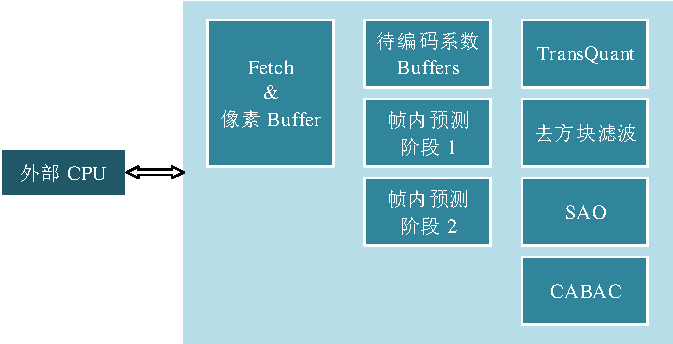
\includegraphics{HardwareArch.pdf}
    \caption{H.265 编码器硬件系统框架}
    \label{fig:HardwareArch}
\end{figure}

图中的外部 CPU 并非系统框架内的模块,系统框架预留了与外部控制器的交互接口,用于进行诸如感兴趣区域 (Range of Interest, ROI)、码率控制、时延控制等外部控制操作。

\section{关键模块的硬件实现}

根据前文所述,H.265 标准下在进行帧内预测时,需要对一个 PU 内的 35 种预测模式进行扫描,从而判断哪种模式是最优的。然而在硬件实现中出现一个问题:在进行预测之前,需要获取其经过重建的参考像素,而参考像素大概率位于前一个 PU 之中,因此,为了等待重建需要让整个预测处理在时序中长时间停留,导致系统吞吐率和硬件的利用率降低,如图 \ref{fig:Intra12}(a) 所示。这一情况在处理大尺寸预测单元时尤为明显。
\begin{figure}[hbt]
    \centering
    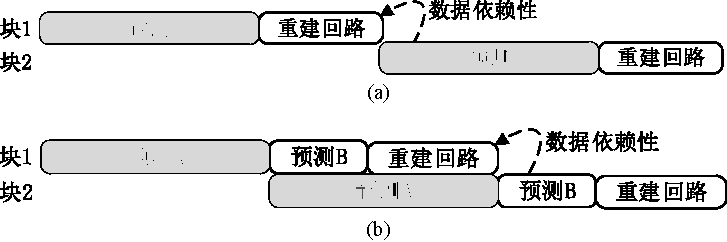
\includegraphics{Intra12.pdf}
    \caption{帧内预测时序说明}
    \label{fig:Intra12}
\end{figure}
基于上述分析,使用了如图 \ref{fig:Intra12}(b) 所示的硬件架构,将预测流程拆分为 2 部分进行:预测 A 使用原始像素而非重建像素作为参考点,来扫描所有的预测模式找出最优的一种,预测 B 与传统预测一致,使用重建像素作为参考点进行预测,但不进行扫描而是使用预测 A 找到的最佳模式直接计算结果,后续的残差计算、熵编码也是以预测 B 的输出结果为准进行的。尽管预测 A 得到的最佳模式可能与标准结果存在出入,但经过大量测试证明该影响可忽略不计,容忍这极少量的编码效率损失可换来更加流畅的系统流水线和更高的吞吐率,显然是值得的。最终该帧内预测模块的顶层结构如图 \ref{fig:Intra12Top} 所示。
\begin{figure}[hbt]
    \centering
    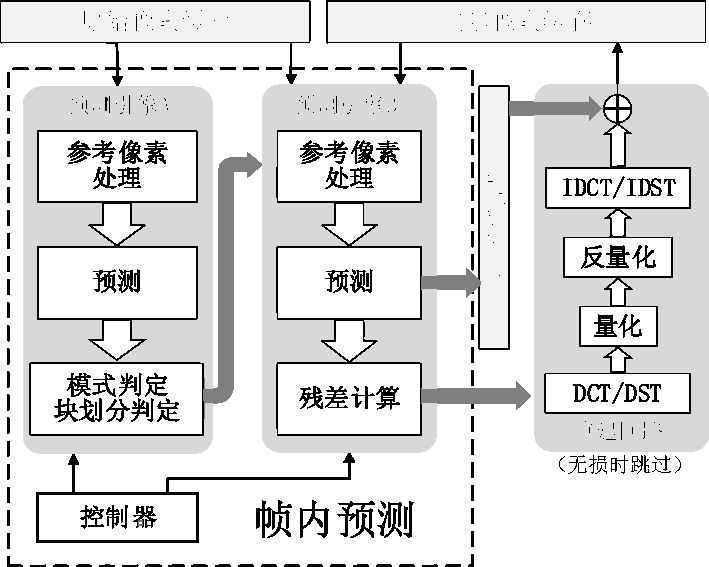
\includegraphics{Intra12Top.pdf}
    \caption{帧内预测模块顶层视图}
    \label{fig:Intra12Top}
\end{figure}



\section{行为级仿真与测试}
% 软件编码结果文件比对
% TSMC 65 nm 400MHz 71+138+764+198+125+103K Logic gate count

\section{本章小结}
本章描述 H.265 帧内无损编码器的 ASIC 实现。介绍了编码器硬件系统架构及其中关键模块的硬件设计,最后给出的行为级仿真验证了编码器的正确性,资源利用报告亦显示该编码器可 ASIC 化。下一章将介绍课题中设计、使用的 FPGA 原型验证平台。